% ------------------------------------------------------------
\section{Calendar Week}
% ------------------------------------------------------------
% --------------------------------------------------- Slide --
\subsection{CW 28}
% ------------------------------------------------------------
\begin{frame}
  \frametitle{Review CW 28}
	\begin{itemize}
		\item "Anerkennung" -> Positive answer from KMK received - \textcolor{green}{Done} 
		\item "Dissertationsanzeige" -> Sent again with updates to "Promotionsbuero" - \textcolor{green}{Done} 
		\item Keys for office at MHH received - \textcolor{green}{Done}
		\item Performed comparison of results between Ansys FEA model and simple Analytical model created with Octave script - \textcolor{green}{Done} 
	\end{itemize}
\end{frame}

\begin{frame}
	\frametitle{Results - Graphics}
	\begin{figure}
	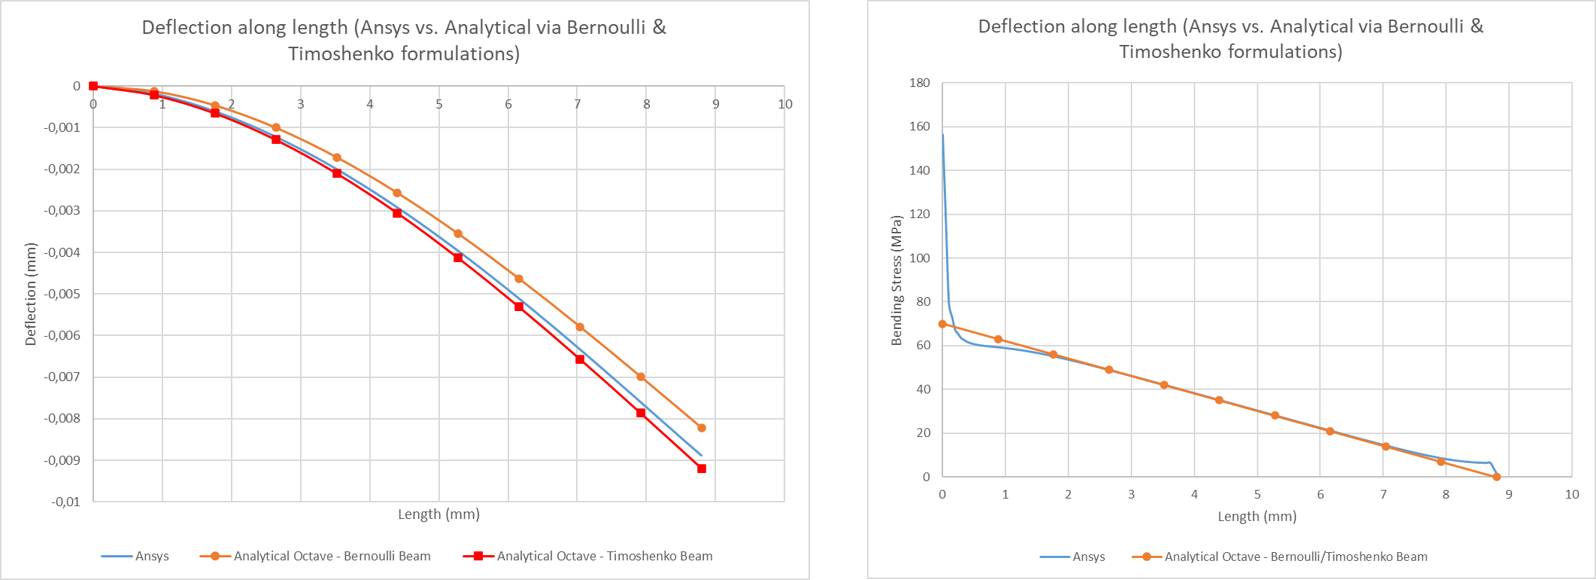
\includegraphics[width=1.0\textwidth]{pictures/CW28_1}
	\caption{Comparison between Ansys and Script (written in Octave) for simple cantilever beam model representing a titanium implant.}
	\end{figure}
\end{frame}

\begin{frame}
  \frametitle{Results - Short discussion}
	\begin{itemize}
		\item Displacement of beam -> Good comparison. First model (Bernoulli beam) with ~10\% difference. Slightly more elaborated model (Timoshenko, considers deformation due to shearing as well, more adequate for short beams as the one used), with 3\% difference to FEA model.
		\item Bending stress of beam -> Good comparison away from the fixed boundary region (same for Bernoulli and Timoshenko analytical models). In the region approximating the fixed boundary there is a significant difference in the results. This is expected for the simplified model (Paper of Augarde2008 has an interesting discussion about the topic).
	\end{itemize}
\end{frame}

% ------------------------------------------------------------
% --------------------------------------------------- Slide --
\subsection{CW 29}
% ------------------------------------------------------------
% ------------------------------------------------------------
\begin{frame}
  \frametitle{Outlook CW 29}
	\begin{itemize}
		\item Add possibility of multi-steps to created script. Objective: calculate and accumulate damage due to different loads in a single run of the script.
	\end{itemize}
\end{frame}
% --------------------------------------------------- Slide --

